\documentclass[a4paper, 11pt]{article}
\usepackage[slovene]{babel}
\usepackage[utf8]{inputenc}
\usepackage{amsmath, amssymb}
\usepackage{graphicx}
\usepackage{float}
\usepackage{caption}
\usepackage{subcaption}
\usepackage{hyperref}
\usepackage{booktabs}
\usepackage{array}
\usepackage{microtype}

\title{Vaja 3 -- LSE, PCA in PCR analiza}
\author{Gašper Leskovec}
\date{\today}

\begin{document}

\maketitle

\section{Uvod}

V nalogi analiziramo identifikacijo modela za proces oksidacije amoniaka v dušikovo kislino
z uporabo treh metod identifikacije:
\begin{itemize}
    \item metoda najmanjših kvadratov (LSE -- Least Squares Estimation),
    \item analiza glavnih komponent (PCA -- Principal Component Analysis),
    \item regresija na glavnih komponentah (PCR -- Principal Component Regression).
\end{itemize}

Vhodne spremenljivke procesa so pretok zraka za hlajenje $A_{FLOW}$, temperatura vode
$T_{H2O}$ in koncentracija kisline $C_{ACID}$, izhodna spremenljivka pa je inverzna
vrednost izkoristka $I_{EFF}$. Ker gre za inverzno vrednost, večja vrednost $I_{EFF}$
pomeni \emph{slabši} izkoristek procesa -- to je treba upoštevati pri branju predznakov
parametrov modela.

Naloga je razdeljena na dva dela:
\begin{itemize}
    \item \textbf{Del 1}: primerjava LSE in PCA glede na vpliv standardizacije podatkov,
    \item \textbf{Del 2}: problem kolinearnosti vhodov in primerjava LSE in PCR kot dveh
    načinov spopadanja z njim.
\end{itemize}

Rezultati v tem poročilu so pridobljeni z MATLAB implementacijo opisane metodologije;
vsi grafi in tabele so generirani neposredno iz izhodov skripte.

\section{Teoretično ozadje}

\subsection{LSE -- metoda najmanjših kvadratov}

Za model z absolutnim (prostim) členom predpostavimo linearno obliko
\[
y = a_1 x_1 + a_2 x_2 + a_3 x_3 + r = \boldsymbol{\varphi}^T \boldsymbol{\theta}
\]
\[
\boldsymbol{\varphi} = [x_1, x_2, x_3, 1]^T,\qquad \boldsymbol{\theta} = [a_1,a_2,a_3,r]^T .
\]
Za $N$ meritev zapišemo $\mathbf{y} = \mathbf{\Phi}\boldsymbol{\theta} + \mathbf{e}$, kjer vrstice
$\mathbf{\Phi}$ vsebujejo $\boldsymbol{\varphi}^T$. Minimizacija vsote kvadratov napak
$J(\boldsymbol{\theta}) = \mathbf{e}^T\mathbf{e}$ vodi do \emph{normalnih enačb}
\[
\mathbf{\Phi}^T\mathbf{\Phi}\,\boldsymbol{\theta} = \mathbf{\Phi}^T\mathbf{y}
\quad\Longrightarrow\quad
\boldsymbol{\theta} = (\mathbf{\Phi}^T\mathbf{\Phi})^{-1}\mathbf{\Phi}^T\mathbf{y}.
\]
LSE minimizira izključno \emph{navpično} (vertikalno) napako v smeri $y$ -- vhodne
spremenljivke $x_i$ obravnava kot brez šuma.

\subsection{PCA -- implicitni model hiperravnine}

Pri PCA v Delu 1 sestavimo razširjeno matriko $\mathbf{Z} = [\mathbf{X}\ \mathbf{y}]$
(vse spremenljivke, vhodi IN izhod, enakovredno). Iz centrirane kovariančne matrike
$\mathbf{F} = \tfrac{1}{N-1}(\mathbf{Z}-\mathbf{v})^T(\mathbf{Z}-\mathbf{v})$ (kjer je
$\mathbf{v}$ vektor povprečij) izračunamo lastne vrednosti in lastne vektorje. Model je
implicitna hiperravnina
\[
\mathbf{p}^T(\mathbf{z} - \mathbf{v}) = 0,
\]
kjer je $\mathbf{p}$ lastni vektor pri \textbf{najmanjši} lastni vrednosti $\mathbf{F}$.
Geometrijsko: $\mathbf{p}$ kaže v smer \emph{najmanjše variance} podatkovnega oblaka
$[\mathbf{X},\mathbf{y}]$ -- to je smer, pravokotno na katero je oblak najbolj "sploščen",
torej normala na ravnino, ki se najbolje prilega podatkom v smislu najmanjše
\emph{pravokotne} (ortogonalne) razdalje. Ta pristop se imenuje tudi
\emph{total least squares} (TLS), ker minimizira napako v VSEH smereh hkrati, ne le v $y$.

Implicitno obliko pretvorimo v eksplicitno z ločitvijo zadnje komponente $p_{n+1}$
(pripadajoče $y$):
\[
a_i = -\frac{p_i}{p_{n+1}},\qquad r = \frac{\mathbf{p}^T\mathbf{v}}{p_{n+1}}
\quad\Longrightarrow\quad y = \mathbf{a}^T\mathbf{x} + r .
\]

\subsection{PCA (Del 1) vs. PCR (Del 2) -- eksplicitna primerjava}
\label{sec:pca-vs-pcr}

Čeprav obe metodi uporabljata isto matematično orodje (lastno razčlenitev /
eigen-dekompozicijo kovariančne matrike), gre za \textbf{dve različni uporabi z nasprotno
logiko izbire lastnega vektorja}, kar eksplicitno strnemo v tabeli~\ref{tab:pca-vs-pcr}.

\begin{table}[H]
\centering
\caption{Eksplicitna primerjava PCA (Del 1) in PCR (Del 2).}
\label{tab:pca-vs-pcr}
\begin{tabular}{@{}p{3cm}p{4.3cm}p{4.3cm}@{}}
\toprule
 & \textbf{PCA (Del 1)} & \textbf{PCR (Del 2)} \\
\midrule
Vhodni podatki & vse spremenljivke $[\mathbf{X},\mathbf{y}]$ & samo vhodi $\mathbf{X}$ (brez $\mathbf{y}$) \\
Izbira lastnega vektorja & \textbf{obdrži} najmanjšo lastno vrednost & \textbf{odstrani} najmanjšo lastno vrednost \\
Vloga izbrane komponente & je normala modela (implicitna ravnina) & se zavrže kot redundantna \\
Regresija & ni potrebna (model je implicitna ravnina) & LSE na preostalih (največjih) komponentah \\
Namen & prileganje total-least-squares & odprava kolinearnosti pred LSE regresijo \\
\bottomrule
\end{tabular}
\end{table}

Pri PCR torej najprej izvedemo PCA na $\mathbf{X}$, odstranimo komponento z najmanjšo
lastno vrednostjo (ki pri kolinearnih vhodih ustreza smeri "redundance" med skoraj
linearno odvisnima spremenljivkama), nato pa izvedemo navadno LSE regresijo v prostoru
preostalih glavnih komponent in parametre preslikamo nazaj v prostor vhodnih
spremenljivk.

\subsection{Numerika: \texttt{inv()} proti operatorju \textbackslash}

Za reševanje linearnega sistema $\mathbf{A}\boldsymbol{\theta}=\mathbf{b}$ (npr. normalnih
enačb) je numerično bolje uporabiti $\boldsymbol{\theta} = \mathbf{A}\backslash\mathbf{b}$
kot $\boldsymbol{\theta} = \mathrm{inv}(\mathbf{A})\mathbf{b}$: operator \textbackslash\
v MATLAB-u izbere ustrezno matrično razčlenitev (npr. Choleskega za simetrično pozitivno
definitno $\mathbf{A}$) in se izogne eksplicitni tvorbi inverza, kar je hitreje in
numerično stabilneje, še posebej če je $\mathbf{A}$ blizu singularne. To postane
pomembno predvsem pri izračunu kovariančne matrike ocenjenih parametrov
($\mathrm{Cov} = \sigma^2 (\mathbf{A})^{-1}$), kjer je $\mathrm{inv}(\mathbf{A})$
nadomeščen z $\mathbf{A}\backslash\mathbf{I}$.

Pomemben diagnostični kazalnik numerične zanesljivosti je \emph{pogojenostno število}
(angl. condition number) $\mathrm{cond}(\mathbf{A}) = \sigma_{\max}(\mathbf{A})/\sigma_{\min}(\mathbf{A})$.
Visoko pogojenostno število ($\gg 1$) pomeni, da je rešitev sistema zelo občutljiva na
majhne motnje v podatkih -- to je natanko simptom kolinearnosti, ki ga obravnavamo v
Delu 2.

\section{Metodologija}

V Delu 1 primerjamo LSE in PCA na treh različnih standardizacijah vhodnih in izhodnih
podatkov: Min-Max na $[0,1]$, Z-score (standardizacija na ničelno povprečje in enotsko
varianco) in brez standardizacije. Modela sta v vsakem primeru ocenjena v
standardiziranem prostoru, nato pa transformirana nazaj v \emph{originalni} prostor
(enote procesa), da je primerjava smiselna in neodvisna od izbrane standardizacije.

V Delu 2 dodamo umetno kolinearno spremenljivko $X_{new} = 2\,T_{H2O} + 6 + \varepsilon$,
$\varepsilon \sim \mathcal{N}(0, 0.1^2)$, standardiziramo vse štiri vhode (Z-score) in
primerjamo LSE (brez prostega člena) s PCR. Eksperiment ponovimo $100$-krat (različni
vzorci šuma $\varepsilon$), da eksperimentalno ocenimo varianco parametrov obeh metod.

\section{Rezultati -- Del 1: vpliv standardizacije}

\subsection{Modeli v originalnem prostoru}

Spodaj so enačbe modelov, izračunane iz ocenjenih parametrov v originalnem prostoru, za
LSE in PCA, pri vseh treh standardizacijah:

\begin{itemize}
    \setlength\itemsep{2pt}
    \item[] LSE, Min-Max: $y = 0.7156\,A_{FLOW} + 1.2953\,T_{H2O} - 0.1521\,C_{ACID} - 39.9197$
    \item[] LSE, Z-Score: $y = 0.7156\,A_{FLOW} + 1.2953\,T_{H2O} - 0.1521\,C_{ACID} - 39.9197$
    \item[] LSE, brez std.: $y = 0.7156\,A_{FLOW} + 1.2953\,T_{H2O} - 0.1521\,C_{ACID} - 39.9197$
    \item[] PCA, Min-Max: $y = 0.7989\,A_{FLOW} + 1.2072\,T_{H2O} - 0.2188\,C_{ACID} - 37.3408$
    \item[] PCA, Z-Score: $y = 0.7988\,A_{FLOW} + 1.2134\,T_{H2O} - 0.2159\,C_{ACID} - 37.7156$
    \item[] PCA, brez std.: $y = 0.4074\,A_{FLOW} + 2.5035\,T_{H2O} - 0.1792\,C_{ACID} - 44.4450$
\end{itemize}

Že na prvi pogled je vidno: LSE parametri so \textbf{identični} pri vseh treh
standardizacijah, PCA parametri pa se \textbf{znatno razlikujejo}, še posebej v primeru
brez standardizacije. To je natančno kvantificirano v razdelku~\ref{sec:robustnost}.

\begin{table}[H]
\centering
\caption{Parametri LSE in PCA modelov v originalnem prostoru.}
\label{tab:part1-params}
\begin{tabular}{lrrrr}
\toprule
Standardizacija & $a_1$ & $a_2$ & $a_3$ & $r$ \\
\midrule
\multicolumn{5}{l}{\textit{LSE}} \\
Min-Max $[0,1]$ & 0.7156 & 1.2953 & $-0.1521$ & $-39.9197$ \\
Z-Score         & 0.7156 & 1.2953 & $-0.1521$ & $-39.9197$ \\
Brez            & 0.7156 & 1.2953 & $-0.1521$ & $-39.9197$ \\
\midrule
\multicolumn{5}{l}{\textit{PCA}} \\
Min-Max $[0,1]$ & 0.7989 & 1.2072 & $-0.2188$ & $-37.3408$ \\
Z-Score         & 0.7988 & 1.2134 & $-0.2159$ & $-37.7156$ \\
Brez            & 0.4074 & 2.5035 & $-0.1792$ & $-44.4450$ \\
\bottomrule
\end{tabular}
\end{table}

\begin{table}[H]
\centering
\caption{Teoretična varianca LSE parametrov v originalnem prostoru (Del 1).}
\label{tab:part1-var}
\begin{tabular}{lrrrr}
\toprule
Standardizacija & $\mathrm{var}(a_1)$ & $\mathrm{var}(a_2)$ & $\mathrm{var}(a_3)$ & $\mathrm{var}(r)$ \\
\midrule
Min-Max $[0,1]$ & 0.018187 & 0.135442 & 0.024428 & 141.5147 \\
Z-Score         & 0.018187 & 0.135442 & 0.024428 & 141.5147 \\
Brez            & 0.018187 & 0.135442 & 0.024428 & 141.5147 \\
\bottomrule
\end{tabular}
\end{table}

Teoretična varianca parametrov je izračunana iz $\mathrm{Cov} = \sigma^2(\mathbf{\Phi}_{std}^T\mathbf{\Phi}_{std})^{-1}$
v standardiziranem prostoru in nato transformirana v originalni prostor. Vrednosti so
\textbf{identične} pri vseh treh standardizacijah -- ne le podobne, temveč do prikazane
natančnosti popolnoma enake. To je neodvisna potrditev iste ugotovitve kot v
razdelku~\ref{sec:robustnost}: LSE je robusten na standardizacijo podatkov, kar se kaže
tako v \emph{enakih ocenjenih parametrih} kot v \emph{enaki teoretični varianci teh
parametrov} -- gre torej za en pojav (afina invariantnost LSE), potrjen z dvema
neodvisnima dokazoma.

\subsection{Napake modelov}

\begin{figure}[H]
\centering
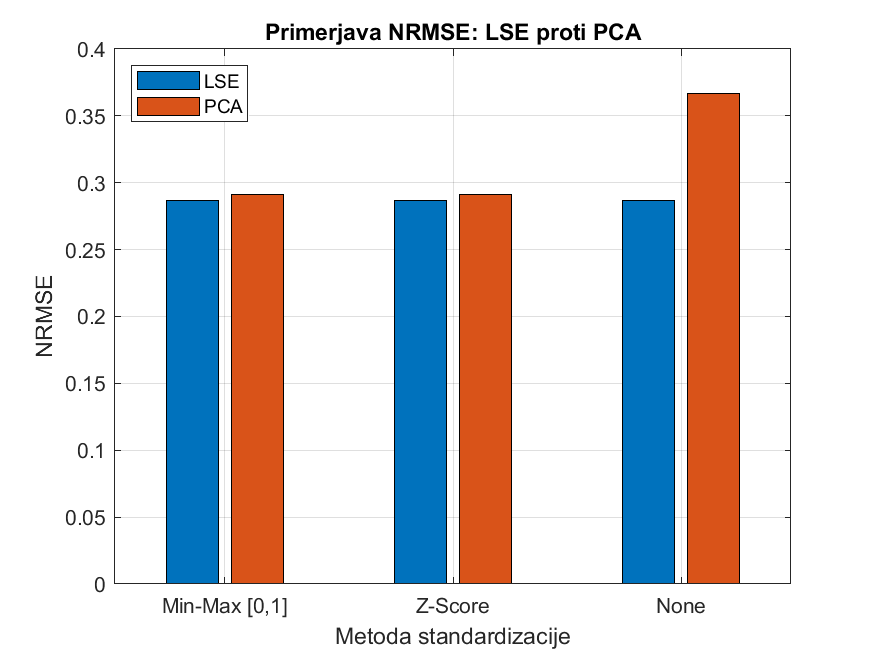
\includegraphics[width=0.8\textwidth]{figs/PART_1_-_NRMSE_comparison.png}
\caption{Primerjava NRMSE: LSE vs. PCA, za vse tri standardizacije.}
\end{figure}

\begin{figure}[H]
\centering
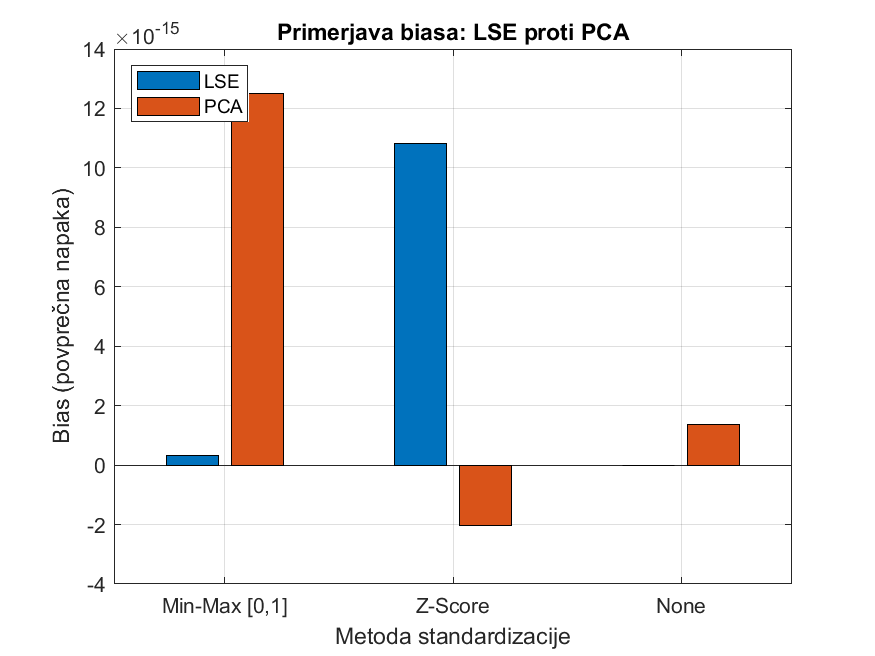
\includegraphics[width=0.8\textwidth]{figs/PART_1_-_Mean_error_comparison.png}
\caption{Primerjava biasa (povprečne napake): LSE vs. PCA.}
\end{figure}

\begin{figure}[H]
\centering
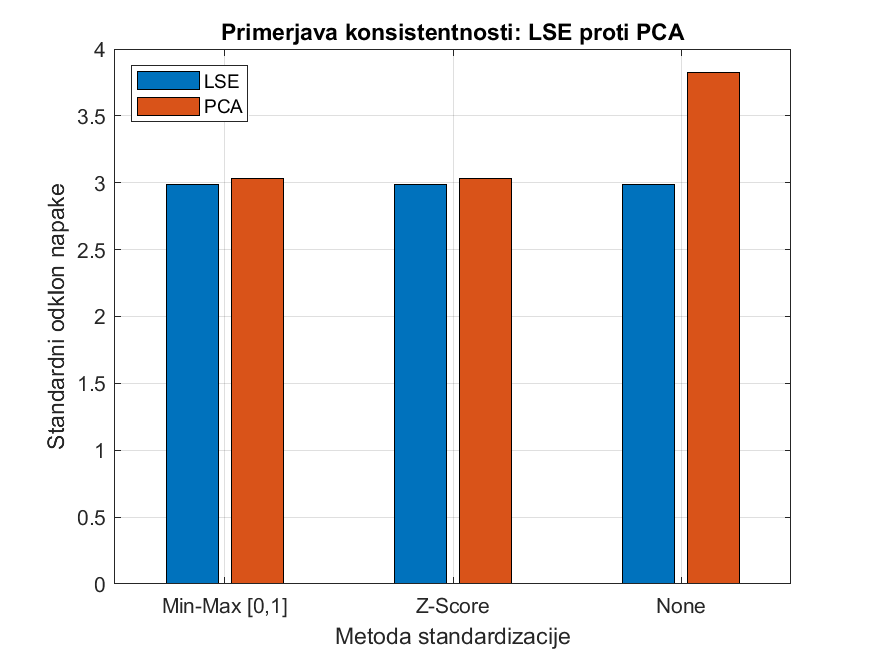
\includegraphics[width=0.8\textwidth]{figs/PART_1_-_Error_standard_deviation_comparison.png}
\caption{Primerjava konsistentnosti (std napake): LSE vs. PCA.}
\end{figure}

\begin{figure}[H]
\centering
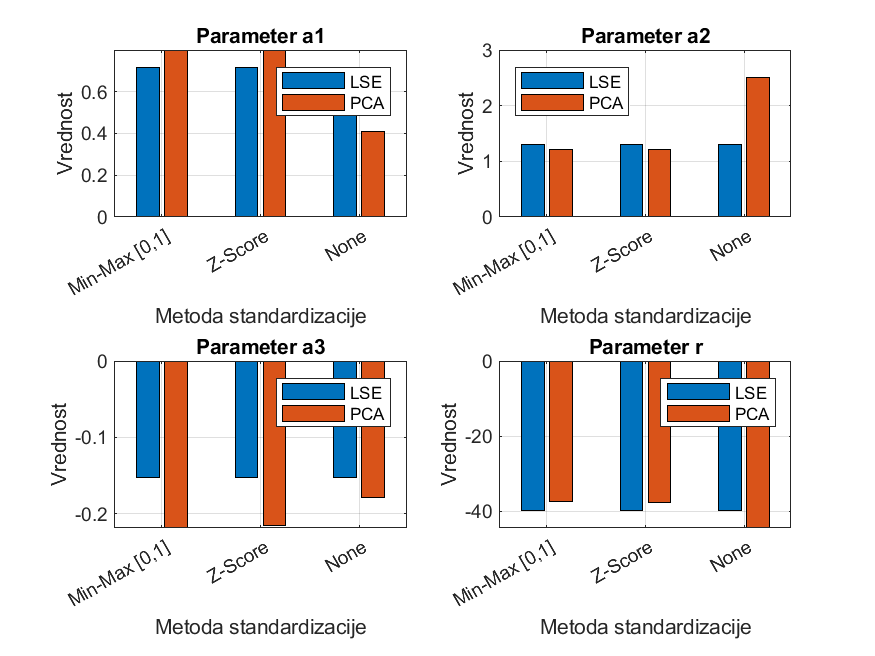
\includegraphics[width=0.8\textwidth]{figs/PART_1_-_Parameter_comparison.png}
\caption{Primerjava vseh štirih parametrov ($a_1,a_2,a_3,r$) med metodama in
standardizacijami.}
\end{figure}

\begin{table}[H]
\centering
\caption{Metrike napake v originalnem prostoru (bias, std napake, NRMSE, ortogonalni RMSE
v standardiziranem prostoru).}
\label{tab:part1-metrics}
\resizebox{\textwidth}{!}{%
\begin{tabular}{lrrrrrrrr}
\toprule
 & \multicolumn{4}{c}{LSE} & \multicolumn{4}{c}{PCA} \\
Standardizacija & bias & std & NRMSE & orthRMSE & bias & std & NRMSE & orthRMSE \\
\midrule
Min-Max & $3.4\times10^{-16}$ & 2.9902 & 0.2869 & 0.0676 & $1.3\times10^{-14}$ & 3.0335 & 0.2910 & 0.0668 \\
Z-Score & $1.1\times10^{-14}$ & 2.9902 & 0.2869 & 0.2279 & $-2.0\times10^{-15}$ & 3.0343 & 0.2911 & 0.2250 \\
Brez    & $0$                & 2.9902 & 0.2869 & 1.6280 & $1.4\times10^{-15}$ & 3.8255 & 0.3670 & 1.3663 \\
\bottomrule
\end{tabular}%
}
\end{table}

\subsection{Porazdelitev napake}
\label{sec:porazdelitev}

Povprečje in standardni odklon povesta le prva dva momenta napake, ne pa njene oblike.
Sliki~\ref{fig:porazdelitev} zato prikazujeta histograma napake $e = y - \hat{y}$ v
originalnem prostoru za LSE in PCA pri standardizaciji z-score.

\begin{figure}[H]
\centering
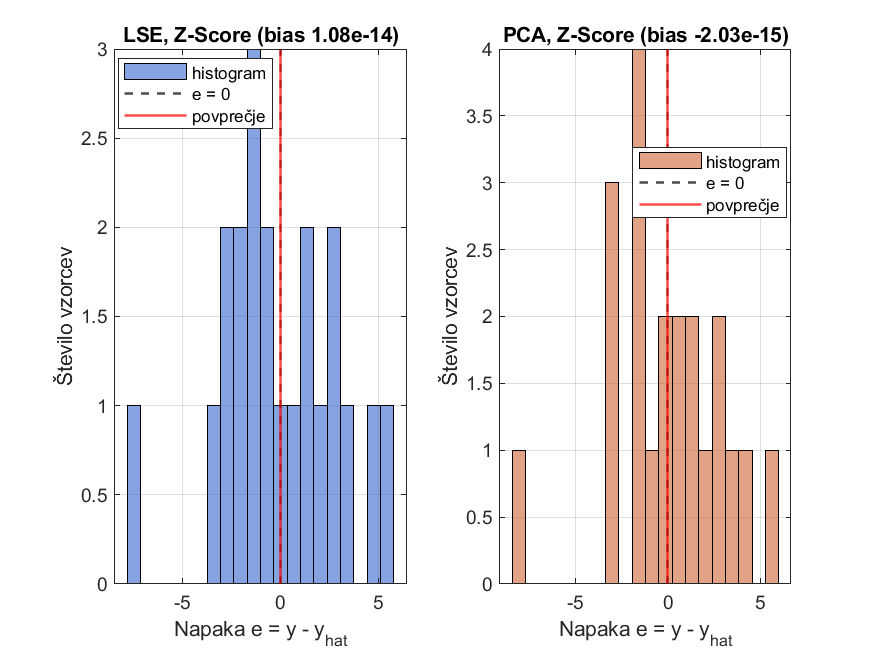
\includegraphics[width=\textwidth]{figs/PART_1_-_Error_distribution.png}
\caption{Porazdelitev napake $e = y - \hat{y}$ v originalnem prostoru pri standardizaciji
z-score, levo LSE, desno PCA. Črtkana črta označuje $e = 0$, polna povprečje napake.}
\label{fig:porazdelitev}
\end{figure}

% TODO: po zagonu kode dopolni opis oblike porazdelitve (simetrija, enovrhost, repi).
Obe porazdelitvi sta centrirani okoli ničle: povprečna napaka znaša $1{,}1\cdot10^{-14}$
pri LSE in $-2{,}0\cdot10^{-15}$ pri PCA, kar je na nivoju numerične natančnosti in
potrjuje, da sta modela nepristranska. Razpršenost je pri obeh primerljiva
(standardni odklon 2{,}9902 pri LSE proti 3{,}0343 pri PCA), kar pomeni, da razlika med
metodama ni v sistematičnem odstopanju, temveč kvečjemu v obliki repov.
% TODO: vstavi vrednost po zagonu -- ali je porazdelitev simetrična in približno normalna
% ali ima izrazitejše repe.
Za nepristranskost je bistveno, da je masa porazdelitve razporejena simetrično okoli
ničle; morebitna asimetrija bi pomenila, da model v določenem delu delovnega območja
sistematično odstopa, česar povprečna napaka blizu nič sama po sebi ne bi razkrila.

\subsection{Diskusija: kaj pove bias in kateri model je boljši?}
\label{sec:bias-discussion}

\textbf{Bias} (pristranskost) je definiran kot povprečna vrednost napake modela,
$\mathrm{bias} = \overline{e} = \overline{y - \hat{y}}$. Vrednost blizu 0 pomeni
nepristranski model -- model v povprečju ne precenjuje ali podcenjuje izhoda.

Iz tabele~\ref{tab:part1-metrics} je razvidno, da je bias \textbf{obeh} modelov (LSE in
PCA), pri \textbf{vseh} treh standardizacijah, reda velikosti $10^{-14}$ do $10^{-16}$ --
to je raven \emph{numeričnega zaokroževanja} plavajoče vejice (float), ne dejanska
modelska razlika. Pravilna interpretacija torej ni "kateri model ima manjši bias" (ker sta
oba praktično enaka in enaka nič), temveč: \textbf{oba modela sta v tem primeru
nepristranska}, kar je pričakovano, saj oba LSE in PCA (implicitni model preko
hiperravnine) po konstrukciji potekata skozi povprečje podatkov. Bias torej v Delu 1
\emph{ni} razlikovalni kriterij med metodama.

Pravi kriterij za izbiro modela sta zato \textbf{std(napake)} (konsistentnost oz. varianca
napake) in \textbf{NRMSE} (normalizirana natančnost). Iz tabele~\ref{tab:part1-metrics}
vidimo, da je LSE pri \emph{vseh treh} standardizacijah enako dober ali boljši od PCA po
obeh teh kriterijih (npr. Min-Max: std $2.9902$ proti $3.0335$, NRMSE $0.2869$ proti
$0.2910$; razlika se še poveča brez standardizacije: std $2.9902$ proti $3.8255$, NRMSE
$0.2869$ proti $0.3670$).

\textbf{Zaključek Dela 1 (utemeljeno priporočilo):} priporočen model je \textbf{LSE} --
ne zaradi biasa (ta ne razlikuje metod), temveč zaradi dosledno manjšega ali enakega
std(napake) in NRMSE pri vseh preizkušenih standardizacijah.

\subsection{Zakaj je PCA po NRMSE "slabši"? -- ni napaka metode}

To ne pomeni, da je PCA slaba ali napačna metoda -- gre za posledico \textbf{drugačnega
kriterija optimizacije}. LSE minimizira izključno \emph{navpično} (vertikalno) napako v
smeri $y$, medtem ko PCA/TLS minimizira \emph{pravokotno} (ortogonalno) napako v skupnem
prostoru $[\mathbf{X},\mathbf{y}]$. NRMSE meri ravno navpično napako -- po TEM kriteriju
je LSE po definiciji vedno enako dober ali boljši, saj je LSE prav ta kriterij eksaktno
minimiziral.

To smo preverili tudi numerično: v tabeli~\ref{tab:part1-metrics} je dodan stolpec
\emph{orthRMSE} -- ortogonalni RMSE do prilegajoče hiperravnine v standardiziranem
prostoru $[\mathbf{X},\mathbf{y}]$. Slika je obratna: pri vseh treh standardizacijah je
PCA po tem (svojem lastnem) kriteriju enako dober ali boljši od LSE (npr. Min-Max:
$0.0668$ proti $0.0676$; brez standardizacije: $1.3663$ proti $1.6280$). To potrjuje, da
noben model ni "napačen" -- gre le za dva različna, veljavna kriterija prileganja.

\subsection{Kvantificirana robustnost LSE in občutljivost PCA na standardizacijo}
\label{sec:robustnost}

V nadaljevanju numerično dokažemo, da je LSE robusten na standardizacijo, PCA pa je
nanjo občutljiv: za vsak parameter ($a_1,a_2,a_3,r$) smo izračunali razpon (max--min, kar je za tri vrednosti
enako maksimalni paroma razliki) med tremi standardizacijami:

\[
\text{LSE razpon} = \max_i\bigl(\theta^{(i)}_{\text{Min-Max}} - \theta^{(i)}_{\text{Z-Score}},\ \ldots\bigr)
\]
\[
\text{LSE razpon} = [1.33\times10^{-15},\ 2.00\times10^{-15},\ 3.41\times10^{-15},\ 3.48\times10^{-13}]
\]
\[
\text{PCA razpon} = [0.3915,\ 1.2964,\ 0.0396,\ 7.1042]
\]

Največja razlika kjerkoli za LSE je $3.48\times10^{-13}$ -- praktično nič (numerični
šum), medtem ko je za PCA največja razlika $7.10$ (parameter $r$) -- za \textbf{13 redov
velikosti} večja. To je neposreden numerični dokaz, da je LSE robusten na
standardizacijo podatkov, PCA pa je nanjo občutljiv.

\emph{Zakaj je temu tako?} LSE minimizira navpično napako, kar je afin-invariantna
lastnost linearne regresije: transformacija $x \to (x-\mathrm{shift})/\mathrm{scale}$ je
afina, zato optimalna rešitev, preslikana nazaj, da isti model ne glede na izbrano
afino transformacijo. PCA pa temelji na relativnih razmerjih varianc med
spremenljivkami (lastne vrednosti kovariančne matrike $[\mathbf{X},\mathbf{y}]$) -- če
spremenljivke niso na primerljivi skali (npr. brez standardizacije, kjer ima $r$ v
originalnih enotah bistveno večjo varianco kot npr. $C_{ACID}$), bo smer najmanjše
variance dominirana s spremenljivko z najmanjšo absolutno varianco, kar ni nujno
smiselna "šumna" smer modela.

\section{Rezultati -- Del 2: problem kolinearnosti}

Dodali smo novo, umetno kolinearno spremenljivko
\[
X_{new} = 2\,T_{H2O} + 6 + \varepsilon,\qquad \varepsilon\sim\mathcal{N}(0,0.1^2).
\]

\subsection{Korelacija}

\begin{figure}[H]
\centering
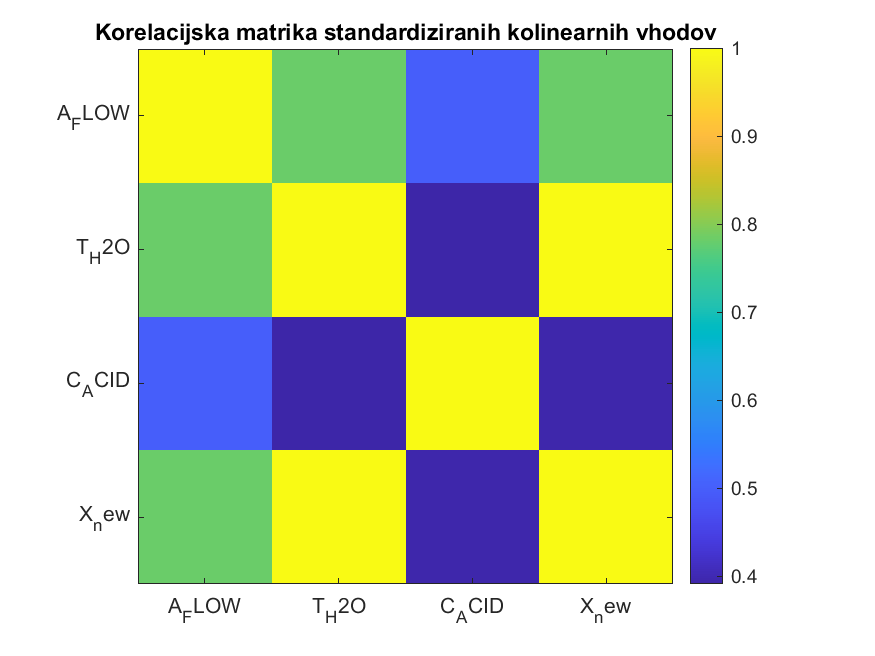
\includegraphics[width=0.6\textwidth]{figs/PART_2_-_Correlation_matrix.png}
\caption{Korelacijska matrika standardiziranih kolinearnih vhodov.}
\end{figure}

\begin{table}[H]
\centering
\caption{Korelacijska matrika standardiziranih vhodov (Del 2).}
\begin{tabular}{lrrrr}
\toprule
 & $A_{FLOW}$ & $T_{H2O}$ & $C_{ACID}$ & $X_{new}$ \\
\midrule
$A_{FLOW}$ & 1.0000 & 0.7819 & 0.5001 & 0.7827 \\
$T_{H2O}$  & 0.7819 & 1.0000 & 0.3909 & 0.9999 \\
$C_{ACID}$ & 0.5001 & 0.3909 & 1.0000 & 0.3940 \\
$X_{new}$  & 0.7827 & 0.9999 & 0.3940 & 1.0000 \\
\bottomrule
\end{tabular}
\end{table}

Korelacija med $T_{H2O}$ in $X_{new}$ je $\mathrm{corr}(T_{H2O}, X_{new}) \approx 0.9999$
-- praktično popolna kolinearnost, kot je bilo pričakovano po konstrukciji $X_{new}$.

\subsection{Parametri modelov -- standardizirani in originalni prostor}

Parametri modelov LSE in PCR so prikazani tako v standardiziranem kot v originalnem
prostoru, saj je slednji edini, v katerem imajo koeficienti neposreden fizikalen pomen.

\textit{Standardiziran prostor (brez prostega člena):}
\begin{itemize}
    \setlength\itemsep{2pt}
    \item[] LSE: $y = 0.6449\,A_{FLOW} + 0.1245\,T_{H2O} - 0.0811\,C_{ACID} + 0.2786\,X_{new}$
    \item[] PCR: $y = 0.6449\,A_{FLOW} + 0.2016\,T_{H2O} - 0.0809\,C_{ACID} + 0.2013\,X_{new}$
\end{itemize}

Opazimo tudi, da PCR koeficienta pri kolinearnem paru ($a_{2} = 0.2016$ za $T_{H2O}$ in
$a_{4} = 0.2013$ za $X_{new}$) med seboj \textbf{skoraj sovpadata} -- PCR torej razdeli
skupni vpliv kolinearnega para praktično enakomerno med obe spremenljivki. LSE tega ne
naredi: njegova koeficienta ($a_2 = 0.1245$, $a_4 = 0.2786$) sta si med seboj precej
različna, saj LSE med kolinearnima vhodoma nima nobenega mehanizma, ki bi vsiljeval
simetrično porazdelitev vpliva.
\textit{Originalni prostor:}
\begin{itemize}
    \setlength\itemsep{2pt}
    \item[] LSE: $y = 0.7154\,A_{FLOW} + 0.4005\,T_{H2O} - 0.1540\,C_{ACID} + 0.4485\,X_{new} - 42.4739$
    \item[] PCR: $y = 0.7155\,A_{FLOW} + 0.6489\,T_{H2O} - 0.1535\,C_{ACID} + 0.3240\,X_{new} - 41.7654$
\end{itemize}

\begin{table}[H]
\centering
\caption{Parametri LSE in PCR (kolinearni primer) v originalnem prostoru.}
\begin{tabular}{lrrrrr}
\toprule
 & $a_1$ & $a_2$ & $a_3$ & $a_4$ & $r$ \\
\midrule
LSE & 0.7154 & 0.4005 & $-0.1540$ & 0.4485 & $-42.4739$ \\
PCR & 0.7155 & 0.6489 & $-0.1535$ & 0.3240 & $-41.7654$ \\
\bottomrule
\end{tabular}
\end{table}

\paragraph{Opažanje: pojav prostega člena po transformaciji.} Modela sta bila v standardiziranem prostoru
ocenjena \textbf{brez} prostega člena ($y_{std} = \mathbf{a}_{std}^T\mathbf{x}_{std}$),
vendar po transformaciji nazaj v originalni prostor dobita \textbf{neničeln} prosti
člen ($r_{\text{LSE}} \approx -42.47$, $r_{\text{PCR}} \approx -41.77$). To ni napaka --
posledica je afinosti standardizacije: ker je z-score transformacija
$x_{std} = (x - \bar{x})/\sigma_x$ afina preslikava z na splošno neničelnim povprečjem
$\bar{x}$, se pri poenostavitvi nazaj v originalne enote pojavi člen
$r_{orig} = \bar{y} - \sum_i a_{orig,i}\,\bar{x}_i$, ki ni nič, razen če je ravno
$\bar{y} = \sum_i a_{orig,i}\bar{x}_i$. "Brez prostega člena" je torej lastnost samo
tega specifičnega (premaknjenega in skaliranega) koordinatnega sistema, ne pa
inherentna lastnost razmerja med $x$ in $y$.

\subsection{Numerika: pogojenostno število -- Del 1 proti Delu 2}

Pogojenostno število matrike normalnih enačb je neposreden pokazatelj (ne)kolinearnosti:

\begin{itemize}
    \item Del 1, Z-Score: $\mathrm{cond}(\mathbf{\Phi}_{std}^T\mathbf{\Phi}_{std}) \approx 1.03\times10^{1}$
    (red velikosti $10^1$ -- dobro pogojena matrika, vhodi so med seboj razmeroma neodvisni).
    \item Del 2, kolinearni primer: $\mathrm{cond}(\mathbf{X}_{col,std}^T\mathbf{X}_{col,std}) \approx 2.47\times10^{4}$
    (red velikosti $10^4$ -- približno \textbf{2400-krat} večje pogojenostno število kot
    v Delu 1).
\end{itemize}

Ta skok za več redov velikosti je numerični podpis kolinearnosti: majhne spremembe v
podatkih (npr. šum $\varepsilon$ v $X_{new}$) se pri reševanju normalnih enačb ojačajo v
veliko večje spremembe ocenjenih parametrov -- kar natanko opazimo pri LSE v naslednjih
razdelkih.

\subsection{Vsota parametrov: standardiziran proti originalnemu prostoru}
\label{sec:vsota}

Ker je $X_{new}$ konstruiran kot $X_{new} = 2\,T_{H2O} + 6 + \varepsilon$, bi
pričakovali, da model "prepozna" to redundanco tako, da je kombiniran prispevek
$T_{H2O}$ in $X_{new}$ podoben prispevku samega $T_{H2O}$ v osnovnem (3-vhodnem) modelu
brez kolinearnosti. Vendar razmerje med $T_{H2O}$ in $X_{new}$ v \textbf{originalnih
enotah} NI 1:1, temveč \textbf{1:2} (zaradi faktorja 2 v definiciji $X_{new}$) -- zato je
treba to preverjanje izvesti pravilno, ločeno v dveh prostorih.

\paragraph{V standardiziranem (z-score) prostoru} preverjanje je neposredno, brez
korekcije, ker z-score standardizacija obe spremenljivki ($T_{H2O}$ in $X_{new}$) skalira
na enotsko varianco -- faktor 2 iz definicije $X_{new}$ se s tem "absorbira" v razmerje
standardnih odklonov in izgine:
\[
a_{2,\text{baseline,std}} = 0.4025
\]
\[
a_{2,\text{LSE,std}} + a_{4,\text{LSE,std}} = 0.1245 + 0.2786 = 0.4031
\]
(za PCR: $0.2016 + 0.2013 = 0.4029$) -- obe vsoti se dobro ujemata z izhodiščno vrednostjo
$0.4025$.

\paragraph{V originalnem prostoru} pa je treba prispevek $X_{new}$ uteži z ustreznim
faktorjem 2, saj $1$ enota $X_{new}$ v originalnih enotah ustreza $2$ enotama $T_{H2O}$:
\[
a_{2,\text{baseline,orig}} = 1.2953 .
\]
\textbf{Brez} korekcije (samo $a_{2,orig}+a_{4,orig}$) se vsoti \textbf{ne ujemata}:
\[
\text{LSE: } 0.4005 + 0.4485 = 0.8490 \quad(\text{razlika od } 1.2953!)
\]
\[
\text{PCR: } 0.6489 + 0.3240 = 0.9729 \quad(\text{razlika od } 1.2953!)
\]
\textbf{S} korekcijo za faktor 2 ($a_{2,orig} + 2\cdot a_{4,orig}$) pa se ujemanje povrne:
\[
\text{LSE: } 0.4005 + 2\cdot 0.4485 = 1.2975 \quad(\approx 1.2953,\ \checkmark)
\]
\[
\text{PCR: } 0.6489 + 2\cdot 0.3240 = 1.2970 \quad(\approx 1.2953,\ \checkmark)
\]

To je netrivialna, a pomembna ugotovitev: preverjanje "vsota parametrov ostane
konstantna" je smiselno in neposredno le v standardiziranem prostoru (kjer
standardizacija implicitno normira razmerje med kolinearnima spremenljivkama), v
originalnem prostoru pa je treba upoštevati dejansko linearno razmerje (tu: faktor 2) iz
definicije kolinearne spremenljivke.

\subsection{Prispevek spremenljivk h glavnim komponentam}

\begin{figure}[H]
\centering
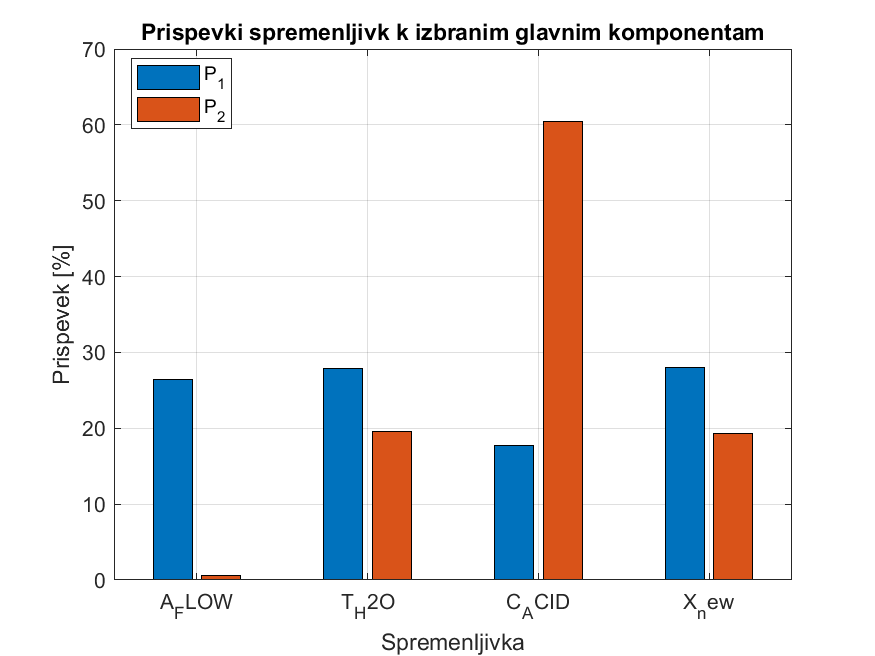
\includegraphics[width=0.8\textwidth]{figs/PART_2_-_PC_contributions.png}
\caption{Prispevki (\%) posameznih vhodnih spremenljivk k prvima dvema (obdržanima)
glavnima komponentama.}
\end{figure}

\begin{table}[H]
\centering
\caption{Prispevki spremenljivk h glavnima komponentama $P_1$ in $P_2$ [\%].}
\begin{tabular}{lrr}
\toprule
 & $P_1$ [\%] & $P_2$ [\%] \\
\midrule
$A_{FLOW}$ & 26.44 & 0.63 \\
$T_{H2O}$  & 27.93 & 19.56 \\
$C_{ACID}$ & 17.68 & 60.49 \\
$X_{new}$  & 27.96 & 19.31 \\
\bottomrule
\end{tabular}
\end{table}

$T_{H2O}$ in $X_{new}$ imata v obeh prikazanih komponentah skoraj identičen prispevek
(27.93~\% proti 27.96~\% v $P_1$, 19.56~\% proti 19.31~\% v $P_2$), kar dodatno potrjuje
njuno kolinearnost -- z vidika PCA sta si spremenljivki praktično neločljivi.

\subsection{Eksperimentalna proti teoretični varianci parametrov}

\begin{figure}[H]
\centering
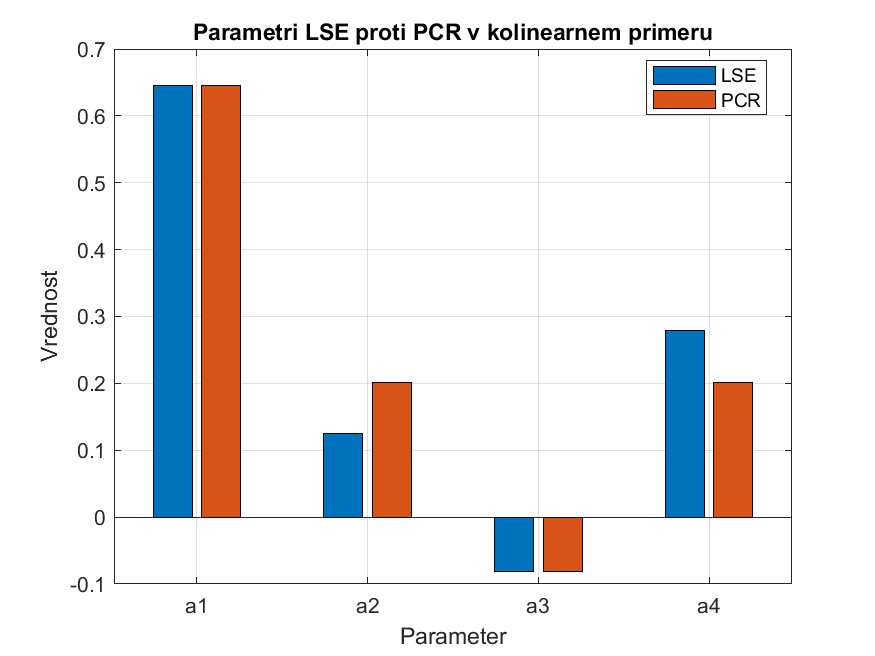
\includegraphics[width=0.8\textwidth]{figs/PART_2_-_Parameter_comparison.png}
\caption{Primerjava parametrov LSE in PCR za en reprezentativen zagon.}
\end{figure}

\begin{figure}[H]
\centering
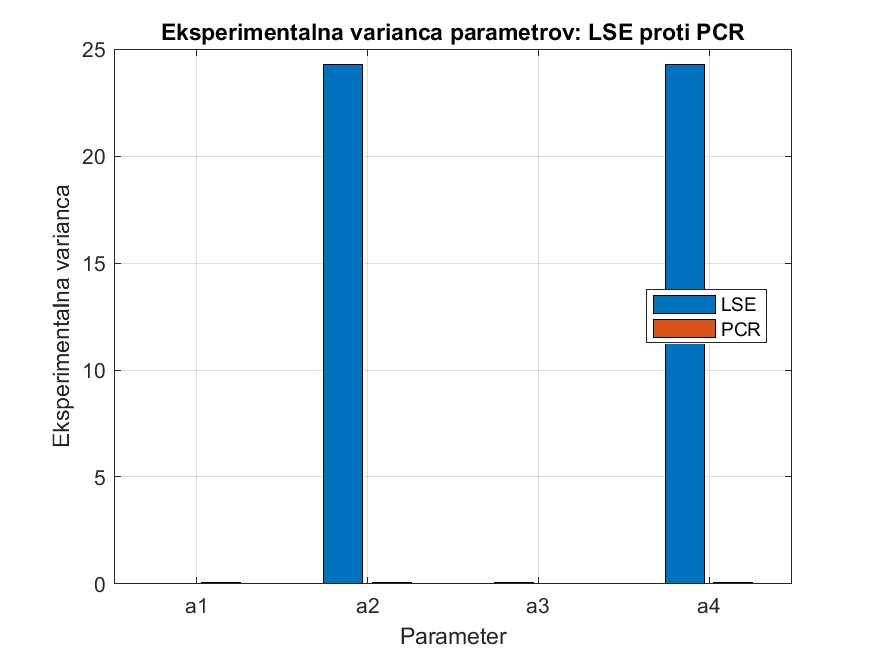
\includegraphics[width=0.8\textwidth]{figs/PART_2_-_Experimental_variance_comparison.png}
\caption{Eksperimentalna varianca parametrov (100 ponovitev) -- LSE proti PCR.}
\end{figure}

\begin{table}[H]
\centering
\caption{Eksperimentalna (100 ponovitev) in teoretična varianca parametrov (kolinearni
primer, standardiziran prostor).}
\begin{tabular}{lrrr}
\toprule
Parameter & LSE (teor. var.) & LSE (eksp. var.) & PCR (eksp. var.) \\
\midrule
$a_1$ & 0.014783  & 0.001026 & $3.01\times10^{-6}$ \\
$a_2$ & 20.985215 & 24.273   & $2.05\times10^{-6}$ \\
$a_3$ & 0.007046  & 0.000218 & $5.32\times10^{-7}$ \\
$a_4$ & 21.058784 & 24.273   & $5.38\times10^{-6}$ \\
\midrule
\textbf{povprečje} & \textbf{10.517} & \textbf{12.137} & \textbf{$2.74\times10^{-6}$} \\
\bottomrule
\end{tabular}
\end{table}

Teoretična varianca LSE parametrov (iz $\mathrm{Cov} = \sigma^2(\mathbf{X}_{col,std}^T\mathbf{X}_{col,std})^{-1}$)
je za $a_2$ in $a_4$ ($20.99$ oz. $21.06$) istega reda velikosti kot eksperimentalno
ocenjena varianca ($24.27$ za oba), kar potrjuje konsistentnost teoretičnega izračuna z
eksperimentom; za $a_1$ in $a_3$ (koeficienta $A_{FLOW}$ in $C_{ACID}$, ki nista udeležena
v kolinearnosti) je teoretična varianca za rede velikosti manjša ($0.0148$ oz. $0.0070$),
prav tako skladno z eksperimentom. Povprečna eksperimentalna varianca LSE parametrov
($12.14$) je za \textbf{približno 6 redov velikosti} večja od povprečne variance PCR
parametrov ($2.74\times10^{-6}$) -- PCR z odstranitvijo redundantne komponente drastično
stabilizira ocenjene parametre.

\subsection{Napaka modela sama po sebi ne razkrije kolinearnosti}

\begin{figure}[H]
\centering
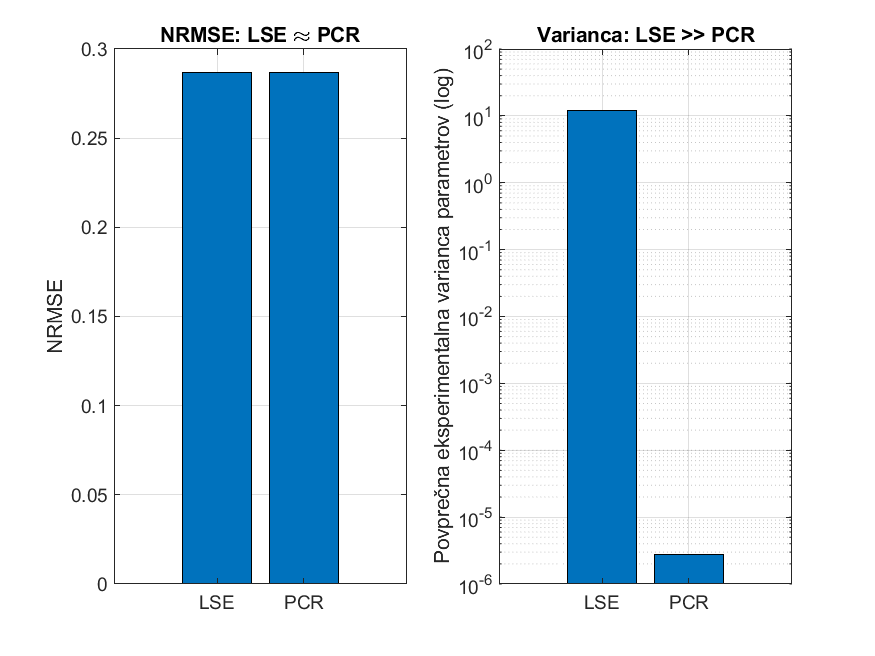
\includegraphics[width=0.8\textwidth]{figs/PART_2_-_Error_vs_Variance.png}
\caption{Levo: NRMSE modela LSE in PCR je praktično enak. Desno: eksperimentalna varianca
parametrov (logaritemska skala) se razlikuje za rede velikosti. Napaka modela torej ne
razkrije problema kolinearnosti -- razkrije ga šele analiza variance/stabilnosti
parametrov.}
\end{figure}

\begin{table}[H]
\centering
\caption{Bias, std napake in NRMSE -- LSE proti PCR, kolinearni primer.}
\begin{tabular}{lrrr}
\toprule
 & bias & std(napaka) & NRMSE \\
\midrule
LSE & $-5.3\times10^{-18}$ & 0.29395 & 0.28686 \\
PCR & $-5.8\times10^{-17}$ & 0.29395 & 0.28686 \\
\bottomrule
\end{tabular}
\end{table}

To je ključna ugotovitev Dela 2: NRMSE LSE ($0.28686$) je \textbf{praktično enak} NRMSE
PCR ($0.28686$) -- gledano samo skozi napako modela na razpoložljivih podatkih, bi
sklepali, da sta modela enakovredna in da ni nobenega problema. Vendar je povprečna
eksperimentalna varianca parametrov LSE ($12.14$) za \textbf{približno 6 redov velikosti}
večja od PCR ($2.74\times10^{-6}$) -- LSE parametri so torej skrajno nestabilni
(majhna sprememba šuma v $X_{new}$ popolnoma spremeni razdelitev prispevka med $T_{H2O}$
in $X_{new}$, glej razdelek~\ref{sec:vsota}), kar iz same napake modela ni razvidno.
\textbf{Zaključek: metrika napake (NRMSE) je nujna, a ne zadostna diagnostika -- za
odkrivanje kolinearnosti je treba analizirati tudi varianco/stabilnost ocenjenih
parametrov} (npr. s ponovljenimi zagoni ali s pogojenostnim številom, glej razdelka
prej).

\section{Zaključek}

Rezultati analize kažejo:

\begin{sloppypar}
\begin{itemize}
    \item V Delu 1 sta LSE in PCA oba nepristranska (bias $\approx 0$, na nivoju
    numeričnega šuma) -- bias torej ni kriterij, ki bi med njima ločil. Ločevalna
    kriterija sta std(napake) in NRMSE, po katerih je LSE dosledno enak ali boljši od
    PCA pri vseh treh standardizacijah -- zato je za ta podatkovni niz priporočen model
    \textbf{LSE}.
    \item LSE je numerično dokazano robusten na izbiro standardizacije
    ($\max|\Delta\theta| \approx 3.5\times10^{-13}$), PCA pa je nanjo občutljiv
    ($\max|\Delta\theta| \approx 7.10$) -- razlog je afina invariantnost LSE v primerjavi
    z PCA, ki temelji na relativnih razmerjih varianc.
    \item PCA ni "slabša" metoda -- le optimizira drugačen (ortogonalni) kriterij od
    NRMSE; to potrjuje uvedena metrika orthRMSE.
    \item V Delu 2 skoraj popolna kolinearnost ($\mathrm{corr}(T_{H2O},X_{new})\approx0.9999$)
    povzroči skok pogojenostnega števila iz reda $10^1$ na red $10^4$ in posledično
    skrajno nestabilne LSE parametre (eksperimentalna varianca $\approx 12.14$).
    \item PCR z odstranitvijo redundantne (najmanjše) glavne komponente pred regresijo
    to nestabilnost odpravi (eksperimentalna varianca $\approx 2.74\times10^{-6}$), ob
    praktično enakem NRMSE kot LSE.
    \item Vsota prispevkov $T_{H2O}$ in $X_{new}$ ostane približno konstantna glede na
    osnovni model \emph{v standardiziranem prostoru neposredno}, v \emph{originalnem}
    prostoru pa šele ob upoštevanju faktorja 2 iz definicije $X_{new}$ -- pomembno
    opozorilo, da se tovrstna preverjanja pravilno izvajajo v prostoru, kjer imajo
    koeficienti neposreden fizikalen pomen.
\end{itemize}
\end{sloppypar}

\textbf{Ključna ugotovitev:}
\begin{quote}
Napaka modela (NRMSE) sama po sebi ne razkrije problema kolinearnosti -- LSE in PCR
dosežeta praktično enak NRMSE, a povsem različno stabilnost ocenjenih parametrov. Za
zanesljivo identifikacijo modela pri (skoraj) kolinearnih vhodih je PCR bistveno boljša
izbira, ker eksplicitno odstrani redundantno smer variance, preden izvede regresijo.
\end{quote}

\end{document}
